% ══════════════════════════════════════════════
% CHƯƠNG 2 — PHÂN TÍCH VÀ THIẾT KẾ CƠ SỞ DỮ LIỆU
% ══════════════════════════════════════════════

\chapter{Phân tích và Thiết kế Cơ sở dữ liệu}

\section{Sơ đồ thực thể mối quan hệ (ERD)}\label{Sec2.1}

Cơ sở dữ liệu \textbf{TravelBookingDB} được thiết kế nhằm xây dựng hệ thống đặt tour du lịch trực tuyến, hỗ trợ quản lý người dùng, tour, lịch khởi hành, đặt chỗ, thanh toán và đánh giá.

Hệ thống bao gồm 14 bảng chính, chia thành các nhóm chức năng:

\begin{itemize}
  \item \textbf{Nhóm người dùng và xác thực:} Accounts, Roles, AccountRoles, CustomerProfiles
  \item \textbf{Nhóm quản lý tour:} Categories, Destinations, Tours, TourSchedules
  \item \textbf{Nhóm nghiệp vụ đặt tour:} Bookings, BookingDetails, Payments, Vouchers
  \item \textbf{Nhóm mở rộng hệ thống:} Reviews, Employees
\end{itemize}

Các bảng được liên kết thông qua khóa chính và khóa ngoại nhằm đảm bảo tính toàn vẹn dữ liệu. Ngoài ra, hệ thống sử dụng các thành phần T-SQL như View, Function, Stored Procedure và Trigger để xử lý nghiệp vụ và tối ưu truy vấn.

\begin{figure}[H]
    \centering
    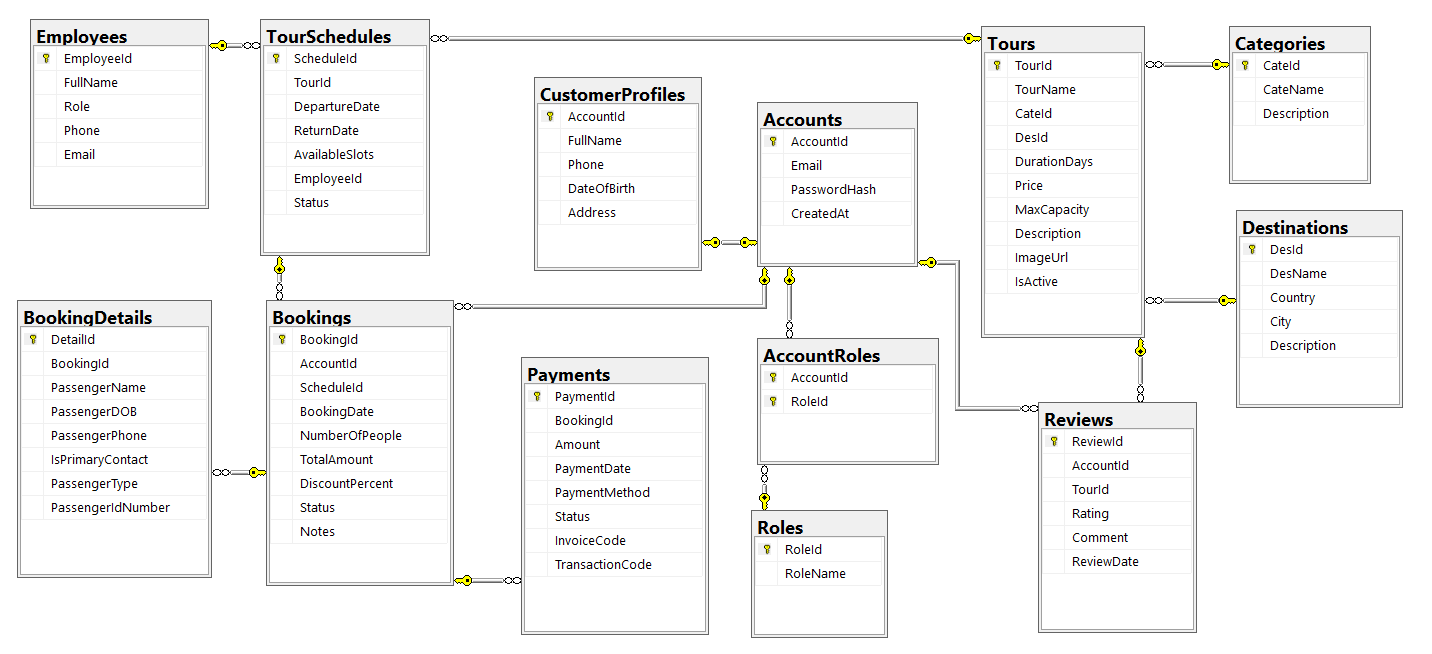
\includegraphics[width=1\linewidth]{image/diagram.png}
    \caption{Sơ đồ thực thể quan hệ database}
    \label{fig:erd}
\end{figure}


% ============================================================
\section{Mô tả các bảng chính}\label{Sec2.2}

\begin{table}[H]
\centering
\begin{tabular}{|l|c|p{8cm}|}
\hline
\textbf{Tên bảng} & \textbf{Số cột} & \textbf{Mô tả} \\
\hline

Categories & 3 & Lưu danh mục tour du lịch như Adventure, Luxury, Family, Beach \\
\hline

Destinations & 5 & Lưu thông tin địa điểm du lịch theo quốc gia, thành phố \\
\hline

Tours & 10 & Quản lý thông tin tour: giá, thời gian, sức chứa, hình ảnh \\
\hline

TourSchedules & 7 & Quản lý lịch khởi hành, số chỗ trống và trạng thái tour \\
\hline

Employees & 5 & Quản lý nhân viên và hướng dẫn viên du lịch \\
\hline

Accounts & 4 & Quản lý tài khoản đăng nhập hệ thống \\
\hline

Roles & 2 & Quản lý vai trò người dùng \\
\hline

AccountRoles & 2 & Phân quyền tài khoản theo vai trò \\
\hline

CustomerProfiles & 5 & Lưu thông tin khách hàng \\
\hline

Bookings & 9 & Quản lý thông tin đặt tour \\
\hline

BookingDetails & 8 & Lưu thông tin hành khách trong mỗi booking \\
\hline

Payments & 8 & Quản lý thanh toán và hóa đơn \\
\hline

Vouchers & 7 & Quản lý mã giảm giá, mức giảm, thời gian hiệu lực và giới hạn lượt sử dụng \\
\hline

Reviews & 6 & Lưu đánh giá và phản hồi tour \\
\hline

\end{tabular}
\caption{Mô tả các bảng trong hệ thống}
\end{table}

% ============================================================
\section{Các ràng buộc dữ liệu}\label{Sec2.3}

Hệ thống áp dụng các ràng buộc nhằm đảm bảo dữ liệu luôn hợp lệ và nhất quán:

\begin{itemize}
  \item Giá tour (Tours.Price) phải lớn hơn 0 
  \item Sức chứa tour (Tours.MaxCapacity) phải lớn hơn 0
  \item Số ngày tour (Tours.DurationDays) phải lớn hơn 0
  \item Ngày về (TourSchedules.ReturnDate) phải lớn hơn ngày đi (DepartureDate)
  \item Số chỗ trống (TourSchedules.AvailableSlots) không được âm
  \item Reviews.Rating chỉ từ 1 đến 5
  \item Số người đi (Bookings.NumberOfPeople) phải lớn hơn 0
  \item Email tài khoản (Accounts và Employees.Email) là duy nhất
  \item Trạng thái booking (Bookings.Status) hợp lệ: Pending, Confirmed, Completed, Cancelled
  \item Trạng thái thanh toán (Payments.Status) hợp lệ: Pending, Completed, Failed, Refunded
  \item Trạng thái lịch tour (TourSchedules.Status): Open, Full, Cancelled
  \item Phần trăm giảm giá (Vouchers.DiscountPercent) nằm trong khoảng từ 0 đến 100
  \item Ngày hết hạn của voucher (Vouchers.EndDate) phải lớn hơn hoặc bằng ngày bắt đầu (Vouchers.StartDate)
  \item Số lượt sử dụng tối đa (Vouchers.MaxUsage) và số lượt đã dùng (Vouchers.UsedCount) không được âm
\end{itemize}

% ============================================================
\section{Views}\label{Sec2.4}

Hệ thống xây dựng 3 View chính phục vụ thống kê và truy vấn dữ liệu.

\noindent\textbf{View 1 — vw\_TourRevenue: thống kê doanh thu và số lượng booking theo từng tour}

\begin{lstlisting}[style=sql, caption={vw\_TourRevenue}]
CREATE VIEW vw_TourRevenue AS
SELECT
T.TourId,
T.TourName,
D.DesName,
COUNT(B.BookingId) AS TotalBookings,
SUM(B.TotalAmount) AS TotalRevenue
FROM Tours T
JOIN Destinations D ON T.DesId = D.DesId
LEFT JOIN TourSchedules S ON T.TourId = S.TourId
LEFT JOIN Bookings B ON S.ScheduleId = B.ScheduleId
AND B.Status IN (N'Confirmed', N'Completed')
GROUP BY T.TourId, T.TourName, D.DesName;
\end{lstlisting}

\noindent\textbf{View 2 — vw\_BookingDetails: xem chi tiết một booking đầy đủ thông tin người đặt và tour}

\begin{lstlisting}[style=sql, caption={vw\_BookingDetails}]
CREATE VIEW vw_BookingDetails AS
SELECT
B.BookingId,
CP.FullName AS UserName,
CP.Phone AS UserPhone,
A.Email AS UserEmail,
T.TourName,
D.DesName,
S.DepartureDate,
S.ReturnDate,
B.NumberOfPeople,
B.TotalAmount,
B.DiscountPercent,
B.Status AS BookingStatus,
B.BookingDate,
B.Notes
FROM Bookings B
JOIN Accounts A ON B.AccountId = A.AccountId
LEFT JOIN CustomerProfiles CP ON A.AccountId = CP.AccountId
JOIN TourSchedules S ON B.ScheduleId = S.ScheduleId
JOIN Tours T ON S.TourId = T.TourId
JOIN Destinations D ON T.DesId = D.DesId;
\end{lstlisting}

\noindent\textbf{View 3 — vw\_PopularTours: xác định tour phổ biến}

\begin{lstlisting}[style=sql, caption={vw\_PopularTours}]
CREATE VIEW vw_PopularTours AS
SELECT
T.TourId,
T.TourName,
T.Price,
T.DurationDays,
C.CateName,
D.DesName,
AVG(CAST(R.Rating AS DECIMAL(3,1))) AS AvgRating,
COUNT(DISTINCT R.ReviewId) AS TotalReviews,
COUNT(DISTINCT B.BookingId) AS BookingCount
FROM Tours T
LEFT JOIN Reviews R ON T.TourId = R.TourId
LEFT JOIN Categories C ON T.CateId = C.CateId
LEFT JOIN Destinations D ON T.DesId = D.DesId
LEFT JOIN TourSchedules S ON T.TourId = S.TourId
LEFT JOIN Bookings B ON S.ScheduleId = B.ScheduleId
AND B.Status IN (N'Confirmed', N'Completed')
GROUP BY T.TourId, T.TourName, T.Price, T.DurationDays, C.CateName, D.DesName;
\end{lstlisting}

% ============================================================
\section{Functions}\label{Sec2.5}

Hệ thống xây dựng 3 hàm T-SQL nhằm hỗ trợ xử lý nghiệp vụ và tối ưu logic trong cơ sở dữ liệu.

% ============================================================
\noindent\textbf{Function 1 — fn\_CalcBookingTotal: Tính tổng tiền booking sau khi áp dụng giảm giá}

\begin{lstlisting}[style=sql, caption={fn\_CalcBookingTotal}]
CREATE FUNCTION fn_CalcBookingTotal(
@ScheduleId INT,
@NumberOfPeople INT,
@DiscountPercent DECIMAL(5,2)
)
RETURNS DECIMAL(12,2)
AS
BEGIN
DECLARE @Price DECIMAL(12,2);
DECLARE @Result DECIMAL(12,2);

SELECT @Price = T.Price
FROM Tours T
JOIN TourSchedules S ON T.TourId = S.TourId
WHERE S.ScheduleId = @ScheduleId;

IF @Price IS NULL
    SET @Result = NULL;
ELSE
    SET @Result = @Price * @NumberOfPeople * (1 - @DiscountPercent / 100);

RETURN @Result;
END;
\end{lstlisting}

% ============================================================
\noindent\textbf{Function 2 — fn\_UserBookingCount: Đếm số lượng booking của khách hàng theo năm}

\begin{lstlisting}[style=sql, caption={fn\_UserBookingCount}]
CREATE FUNCTION fn_UserBookingCount(
@AccountId INT,
@Year INT
)
RETURNS INT
AS
BEGIN
DECLARE @Count INT;

SELECT @Count = COUNT(*)
FROM Bookings
WHERE AccountId = @AccountId
  AND YEAR(BookingDate) = @Year
  AND Status != N'Cancelled';

RETURN ISNULL(@Count, 0);
END;
\end{lstlisting}

% ============================================================
\noindent\textbf{Function 3 — fn\_GenerateInvoiceCode: Sinh mã hóa đơn theo định dạng INV-YYYY-XXXX}

\begin{lstlisting}[style=sql, caption={fn\_GenerateInvoiceCode}]
CREATE FUNCTION fn_GenerateInvoiceCode(@BookingId INT)
RETURNS NVARCHAR(50)
AS
BEGIN
DECLARE @Year NVARCHAR(4) = CAST(YEAR(GETDATE()) AS NVARCHAR(4));
DECLARE @Seq  NVARCHAR(4) = RIGHT('0000' + CAST(@BookingId AS NVARCHAR(10)), 4);
RETURN N'INV-' + @Year + N'-' + @Seq;
END;
\end{lstlisting}

% ============================================================
\section{Stored Procedures}\label{Sec2.6}

Hệ thống xây dựng các Stored Procedure nhằm xử lý nghiệp vụ chính như đặt tour, hủy tour, tìm kiếm tour và báo cáo doanh thu. Các procedure này đảm bảo tính toàn vẹn dữ liệu thông qua cơ chế transaction và kiểm tra điều kiện dữ liệu đầu vào.

% ============================================================
\subsection{sp\_CreateBooking}

Stored Procedure \textbf{sp\_CreateBooking} là nghiệp vụ quan trọng nhất của hệ thống, dùng để thực hiện chức năng đặt tour và kiểm soát số lượng chỗ trống theo thời gian thực.

\begin{lstlisting}[style=sql, caption={sp\_CreateBooking}]
CREATE PROCEDURE sp_CreateBooking
@AccountId INT,
@ScheduleId INT,
@NumberOfPeople INT,
@DiscountPercent DECIMAL(5,2)
AS
BEGIN
SET NOCOUNT ON;

IF NOT EXISTS (SELECT 1 FROM TourSchedules WHERE ScheduleId = @ScheduleId)
    THROW 50001, N'Không tìm thấy lịch khởi hành', 1;

IF NOT EXISTS (SELECT 1 FROM Accounts WHERE AccountId = @AccountId)
    THROW 50002, N'Không tìm thấy khách hàng', 1;

BEGIN TRY
    BEGIN TRANSACTION;

    DECLARE @Available INT;

    SELECT @Available = AvailableSlots
    FROM TourSchedules WITH (UPDLOCK, ROWLOCK)
    WHERE ScheduleId = @ScheduleId;

    IF @Available < @NumberOfPeople
        THROW 50003, N'Không đủ chỗ trống', 1;

    DECLARE @Total DECIMAL(12,2);
    SET @Total = dbo.fn_CalcBookingTotal(@ScheduleId, @NumberOfPeople, @DiscountPercent);

    IF @Total IS NULL
        THROW 50004, N'Không thể tính giá tour', 1;

    INSERT INTO Bookings (AccountId, ScheduleId, NumberOfPeople, TotalAmount, DiscountPercent, Status)
    VALUES (@AccountId, @ScheduleId, @NumberOfPeople, @Total, @DiscountPercent, N'Confirmed');

    COMMIT;

    SELECT SCOPE_IDENTITY() AS NewBookingId;

END TRY
BEGIN CATCH
    IF @@TRANCOUNT > 0 ROLLBACK;
    THROW;
END CATCH
END;
\end{lstlisting}

% ============================================================
\subsection{sp\_CancelBooking}

Stored Procedure \textbf{sp\_CancelBooking} dùng để hủy booking hợp lệ, đồng thời kiểm tra trạng thái hiện tại của đơn đặt.

\begin{lstlisting}[style=sql, caption={sp\_CancelBooking}]
CREATE PROCEDURE sp_CancelBooking
@BookingId INT
AS
BEGIN
SET NOCOUNT ON;

DECLARE @CurrentStatus NVARCHAR(50);
SELECT @CurrentStatus = Status FROM Bookings WHERE BookingId = @BookingId;

IF @CurrentStatus IS NULL
    THROW 50005, N'Không tìm thấy booking', 1;

IF @CurrentStatus = N'Cancelled'
    THROW 50006, N'Booking đã được hủy trước đó', 1;

IF @CurrentStatus = N'Completed'
    THROW 50007, N'Không thể hủy booking đã hoàn thành', 1;

BEGIN TRY
    BEGIN TRANSACTION;

    UPDATE Bookings
    SET Status = N'Cancelled'
    WHERE BookingId = @BookingId;

    COMMIT;
END TRY
BEGIN CATCH
    IF @@TRANCOUNT > 0 ROLLBACK;
    THROW;
END CATCH

END;
\end{lstlisting}

% ============================================================
\subsection{sp\_SearchTours}

Stored Procedure \textbf{sp\_SearchTours} hỗ trợ tìm kiếm tour theo nhiều điều kiện như điểm đến, khoảng giá và ngày khởi hành.

\begin{lstlisting}[style=sql, caption={sp\_SearchTours}]
CREATE PROCEDURE sp_SearchTours
@Destination NVARCHAR(100) = NULL,
@PriceMin DECIMAL(12,2) = NULL,
@PriceMax DECIMAL(12,2) = NULL,
@Date DATE = NULL
AS
BEGIN
SET NOCOUNT ON;

SELECT
    T.TourId, T.TourName, T.Price, T.DurationDays,
    T.MaxCapacity, T.Description, T.ImageUrl,
    D.DesName, D.Country,
    S.ScheduleId, S.DepartureDate, S.ReturnDate,
    S.AvailableSlots, S.Status AS ScheduleStatus
FROM Tours T
JOIN Destinations D ON T.DesId = D.DesId
JOIN TourSchedules S ON T.TourId = S.TourId
WHERE T.IsActive = 1
  AND S.AvailableSlots > 0
  AND S.Status = N'Open'
  AND (@Destination IS NULL OR D.DesName LIKE N'%' + @Destination + N'%')
  AND (@PriceMin IS NULL OR T.Price >= @PriceMin)
  AND (@PriceMax IS NULL OR T.Price <= @PriceMax)
  AND (@Date IS NULL OR S.DepartureDate >= @Date)
ORDER BY S.DepartureDate;

END;
\end{lstlisting}

% ============================================================
\subsection{sp\_RevenueReport}

Stored Procedure \textbf{sp\_RevenueReport} dùng để thống kê doanh thu theo tháng và năm.

\begin{lstlisting}[style=sql, caption={sp\_RevenueReport}]
CREATE PROCEDURE sp_RevenueReport
@FromDate DATE = NULL,
@ToDate DATE = NULL
AS
BEGIN
SET NOCOUNT ON;

SELECT
    YEAR(BookingDate) AS RevenueYear,
    MONTH(BookingDate) AS RevenueMonth,
    COUNT(BookingId) AS TotalBookings,
    SUM(TotalAmount) AS TotalRevenue,
    AVG(TotalAmount) AS AvgOrderValue
FROM Bookings
WHERE Status IN (N'Confirmed', N'Completed')
  AND (@FromDate IS NULL OR CAST(BookingDate AS DATE) >= @FromDate)
  AND (@ToDate IS NULL OR CAST(BookingDate AS DATE) <= @ToDate)
GROUP BY YEAR(BookingDate), MONTH(BookingDate)
ORDER BY RevenueYear, RevenueMonth;
END;
\end{lstlisting}

% ============================================================
\section{Triggers}\label{Sec2.7}

Trigger tự động cập nhật số chỗ khi có booking mới hoặc hủy booking.

\begin{lstlisting}[style=sql, caption={trg\_AfterBookingInsert}]
CREATE TRIGGER trg_AfterBookingInsert
ON Bookings
AFTER INSERT
AS
BEGIN
SET NOCOUNT ON;

UPDATE TS
SET TS.AvailableSlots = TS.AvailableSlots - I.NumberOfPeople
FROM TourSchedules TS
JOIN inserted I ON TS.ScheduleId = I.ScheduleId;

UPDATE TS
SET TS.Status = N'Full'
FROM TourSchedules TS
JOIN inserted I ON TS.ScheduleId = I.ScheduleId
WHERE TS.AvailableSlots = 0;

END;
\end{lstlisting}

\begin{lstlisting}[style=sql, caption={trg\_AfterBookingCancel}]
CREATE TRIGGER trg_AfterBookingCancel
ON Bookings
AFTER UPDATE
AS
BEGIN
SET NOCOUNT ON;

IF UPDATE(Status)
BEGIN
    UPDATE TS
    SET TS.AvailableSlots = TS.AvailableSlots + I.NumberOfPeople
    FROM TourSchedules TS
    JOIN inserted I ON TS.ScheduleId = I.ScheduleId
    JOIN deleted D ON D.BookingId = I.BookingId
    WHERE I.Status = N'Cancelled'
      AND D.Status != N'Cancelled';

    UPDATE TS
    SET TS.Status = N'Open'
    FROM TourSchedules TS
    JOIN inserted I ON TS.ScheduleId = I.ScheduleId
    WHERE I.Status = N'Cancelled'
      AND TS.AvailableSlots > 0
      AND TS.Status = N'Full';
END

END;
\end{lstlisting}



\renewcommand{\thefigure}{2.8.\arabic{figure}}
\setcounter{figure}{0}% ============================================================
\section{Kết quả kiểm thử T-SQL}\label{Sec2.8}

TEST 1 — Tạo booking hợp lệ:
\begin{itemize}
  \item Kiểm tra Stored Procedure sp\_CreateBooking
  \item Kiểm tra trigger tự động giảm AvailableSlots
\end{itemize}

\begin{figure}[H]
    \centering
    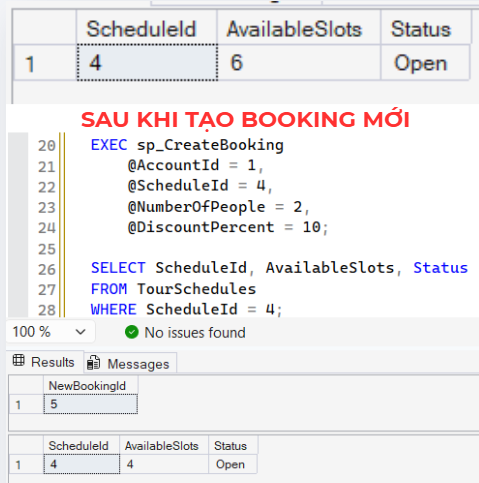
\includegraphics[width=1\linewidth]{image/test1.png}
    \caption{Kiểm thử tạo booking}
    \label{fig:placeholder}
\end{figure}


TEST 2 — Không đủ chỗ trống: Kiểm tra validate slot
\begin{figure}[H]
    \centering
    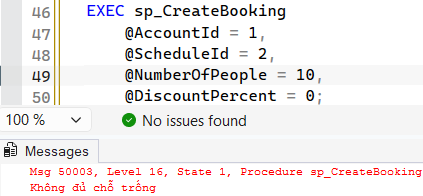
\includegraphics[width=1\linewidth]{image/test2.png}
    \caption{Kiểm thử validate slot}
    \label{fig:placeholder}
\end{figure}

TEST 3 — Tạo booking nhưng Schedule không tồn tại
\begin{figure}[H]
    \centering
    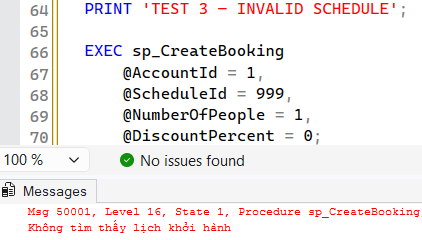
\includegraphics[width=1\linewidth]{image/test3.png}
    \caption{Tạo booking nhưng Schedule không tồn tại}
    \label{fig:placeholder}
\end{figure}

TEST 4 — Hủy booking hợp lệ:
\begin{itemize}
  \item Kiểm tra sp\_CancelBooking
  \item Trigger tự cộng lại slot
\end{itemize}

\begin{figure}[H]
    \centering
    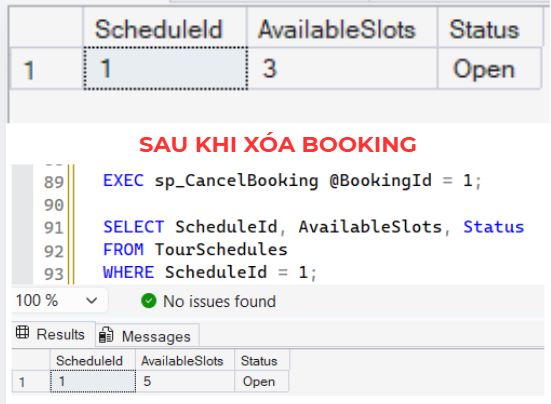
\includegraphics[width=1\linewidth]{image/test4.png}
    \caption{Kiểm tra hủy booking hợp lệ}
    \label{fig:placeholder}
\end{figure}

TEST 5 — Hủy booking đã hủy trước đó
\begin{figure}[H]
    \centering
    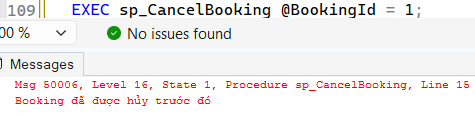
\includegraphics[width=1\linewidth]{image/test5.png}
    \caption{Kiểm tra hủy booking đã hủy trước đó}
    \label{fig:placeholder}
\end{figure}

TEST 6 — Tìm kiếm tour theo điểm đến
\begin{figure}[H]
    \centering
    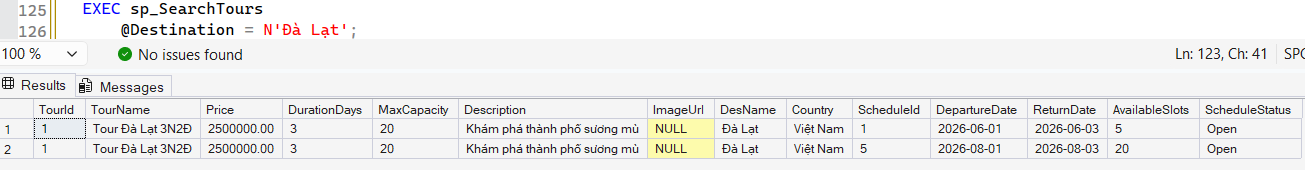
\includegraphics[width=1\linewidth]{image/test6.png}
    \caption{Kiểm tra Tìm kiếm tour theo điểm đến}
    \label{fig:placeholder}
\end{figure}

TEST 7 — Tìm kiếm tour theo khoảng giá
\begin{figure}[H]
    \centering
    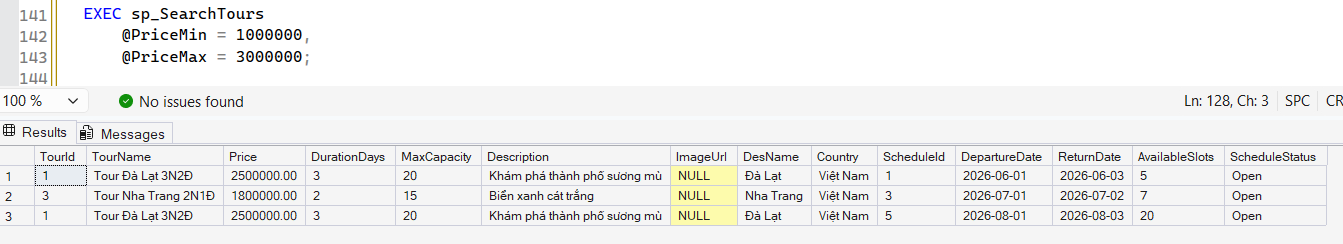
\includegraphics[width=1\linewidth]{image/test7.png}
    \caption{Kiểm tra Tìm kiếm tour theo khoảng giá}
    \label{fig:placeholder}
\end{figure}

TEST 8 — Kiểm tra View vw\_TourRevenue : Hiển thị tổng booking và doanh thu từng tour
\begin{figure}[H]
    \centering
    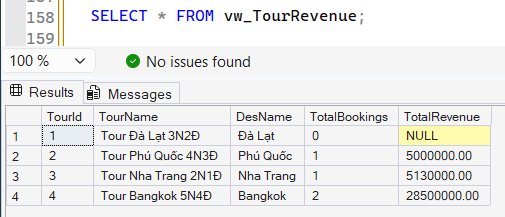
\includegraphics[width=1\linewidth]{image/test8.png}
    \caption{Kiểm tra View vw\_TourRevenue}
    \label{fig:placeholder}
\end{figure}

TEST 9 — Kiểm tra View vw\_BookingDetails: Hiển thị đầy đủ thông tin booking, khách hàng và tour
\begin{figure}[H]
    \centering
    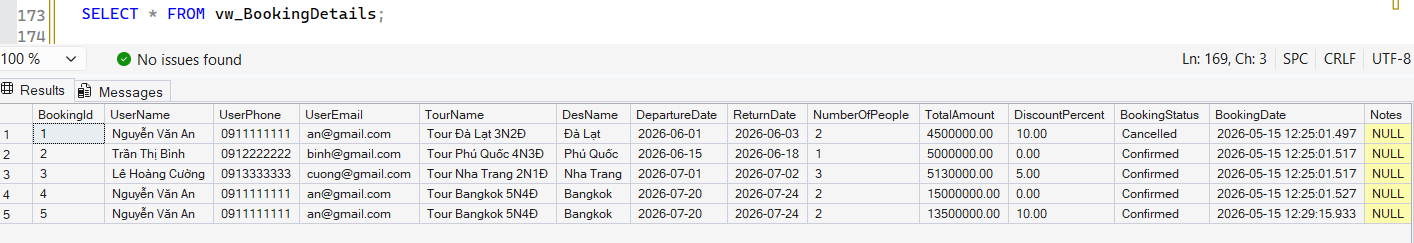
\includegraphics[width=1\linewidth]{image/test9.png}
    \caption{Kiểm tra View vw\_BookingDetails}
    \label{fig:placeholder}
\end{figure}

TEST 10 — Kiểm tra View vw\_PopularTours: Hiển thị rating trung bình, số review và booking
\begin{figure}[H]
    \centering
    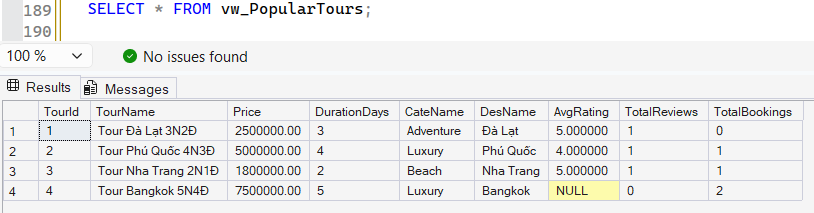
\includegraphics[width=1\linewidth]{image/test10.png}
    \caption{Kiểm tra View vw\_PopularTours}
    \label{fig:placeholder}
\end{figure}

TEST 11 — Kiểm tra Function fn\_CalcBookingTotal: Trả về Tổng tiền = Giá tour × số người × giảm giá
\begin{figure}[H]
    \centering
    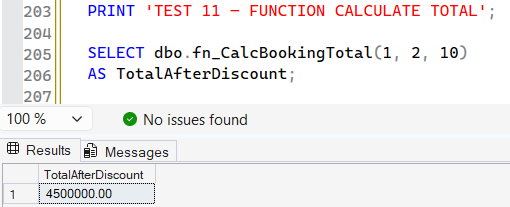
\includegraphics[width=1\linewidth]{image/test11.png}
    \caption{Kiểm tra Function fn\_CalcBookingTotal}
    \label{fig:placeholder}
\end{figure}

TEST 12 — Kiểm tra Function fn\_UserBookingCount: Đếm tổng booking dựa vào AccountId và năm
\begin{figure}[H]
    \centering
    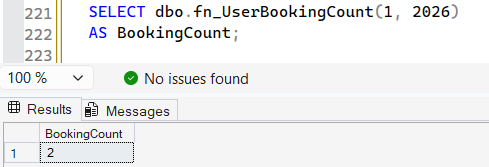
\includegraphics[width=1\linewidth]{image/test12.png}
    \caption{Kiểm tra Function fn\_UserBookingCount}
    \label{fig:placeholder}
\end{figure}

TEST 13 — Kiểm tra Function fn\_GenerateInvoiceCode: Hàm sinh InvoiceCode
\begin{figure}[H]
    \centering
    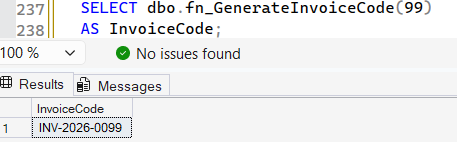
\includegraphics[width=1\linewidth]{image/test13.png}
    \caption{Kiểm tra Function fn\_GenerateInvoiceCode}
    \label{fig:placeholder}
\end{figure}

TEST 14 — Báo cáo doanh thu
\begin{figure}[H]
    \centering
    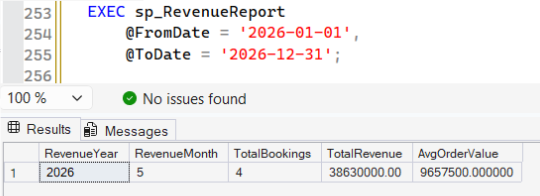
\includegraphics[width=1\linewidth]{image/test14.png}
    \caption{Kiểm tra hàm báo cáo doanh thu}
    \label{fig:placeholder}
\end{figure}

TEST 15 — Trigger tự chuyển trạng thái Full: Đặt booking liên tục đến khi hết slot
\begin{figure}[H]
    \centering
    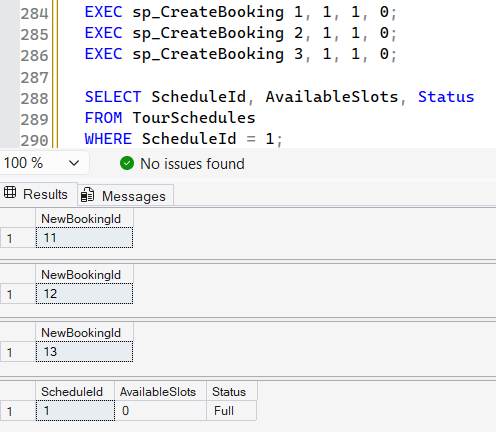
\includegraphics[width=1\linewidth]{image/test15.png}
    \caption{Kiểm tra trigger liên tục}
    \label{fig:placeholder}
\end{figure}

TEST 16 — Không thể đặt thêm khi đã Full: Trả về "Không đủ chỗ trống"
\begin{figure}[H]
    \centering
    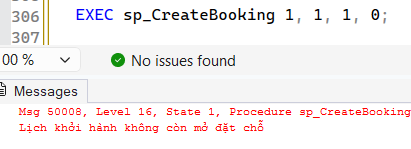
\includegraphics[width=1\linewidth]{image/test16.png}
    \caption{Kiểm tra booking khi "Không đủ chỗ trống"}
    \label{fig:placeholder}
\end{figure}
